\chapter{基于孪生网络的隐藏需求挖掘方法}
% 上文中介绍的p-{\tool}可以对单个对话进行建模并进行分类,但由于数据标注困难的问题,p-{\tool}模型存在着训练数据不足的问题。针对这个问题,
本章介绍了本文设计的{\tool}方法,其总体框架如图\ref{fig:approach}所示,{\tool}以第3章中设计的两个相同上下文敏感对话模型为基模型构建了一个孪生网络,并构建Pair-Instance作为{\tool}的输入样本,分类目标为输入的两个对话是否为相同的类别。在获取{\tool}对输入的两个对话是否为相同类别的预测之后,{\tool}基于此预测结果和配对实例中已标注对话的实际标签来推断目标对话的预测类别,以达到对对话进行分类的目的,从而可以进行需求识别。
\begin{figure}[htbp]
    \centering
    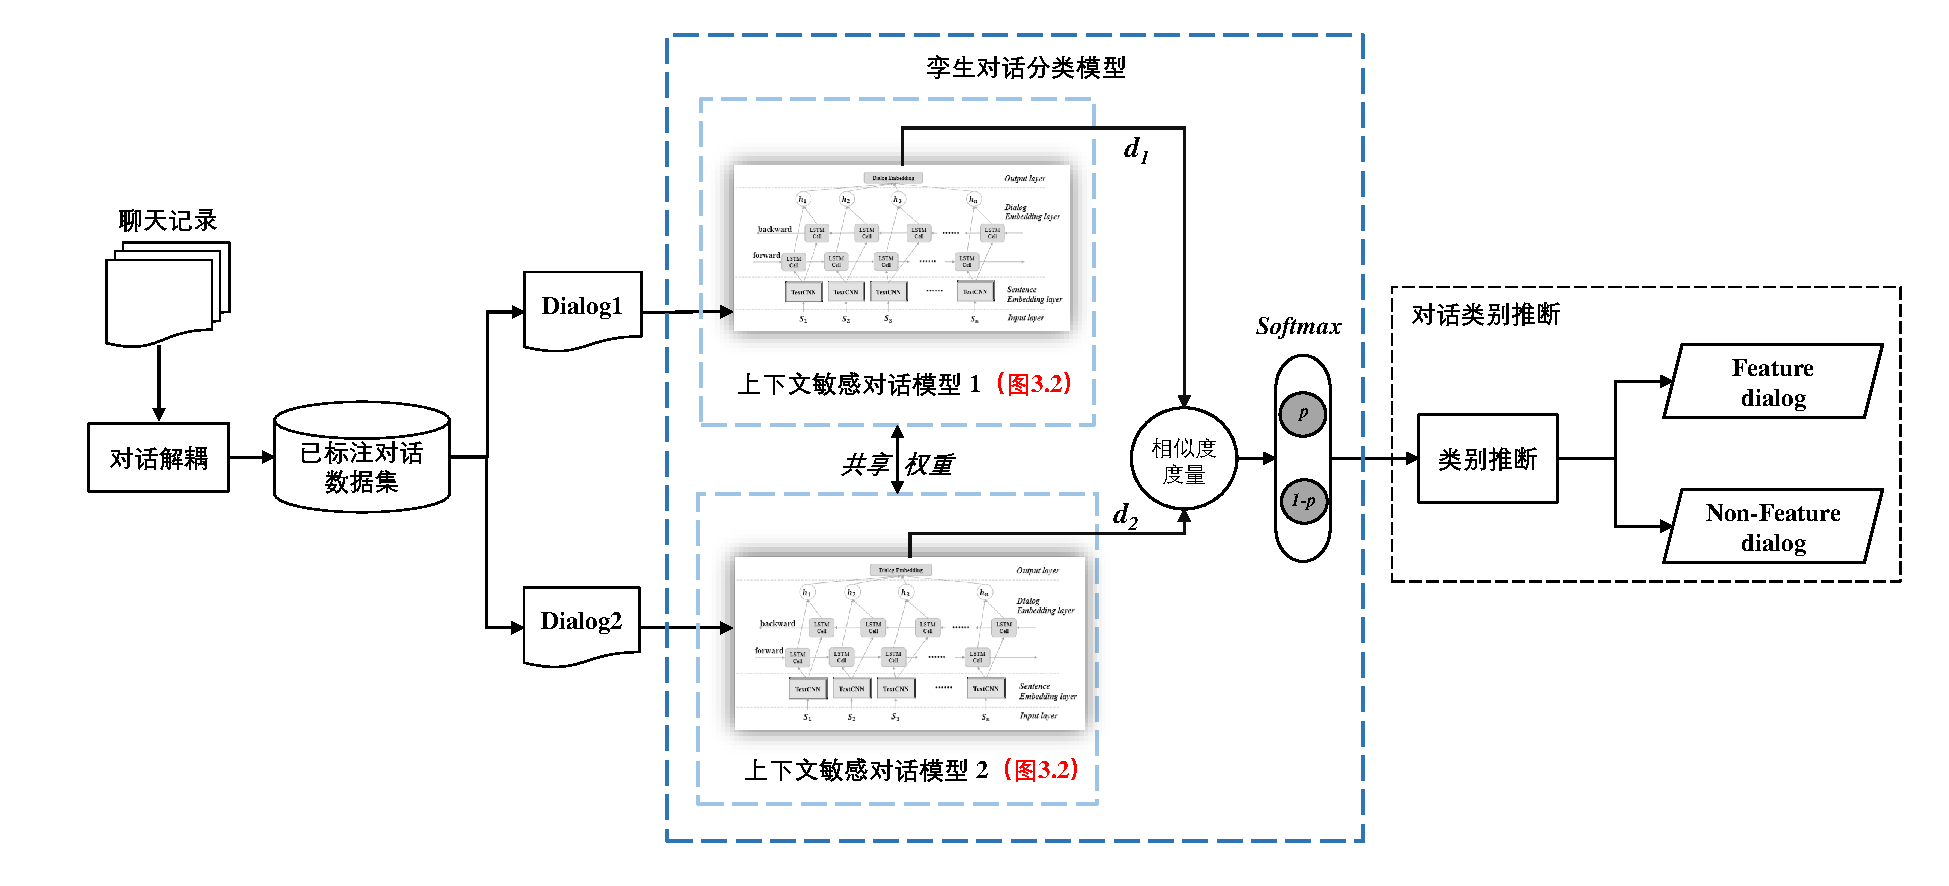
\includegraphics[width=\textwidth]{Img/approach.pdf}
    \bicaption{FRMiner模型结构图}{Architecture of FRMiner}
    \label{fig:approach}
\end{figure}


\section{{\tool}模型结构设计}
为了缓解标注数据不足的问题,本文构建了对话分类孪生网络,传统的文本分类方法将单个对话映射到其类别,本文则将其转换为确定两个对话是否属于同一类的任务,同时可以扩充数据集。为了清楚起见,在下文中,将使用\textit{feature dialog}和\textit{non-feature dialog}来表示为需求意图的对话和不是需求意图的对话。

图\ref{fig:approach}中标识Siamese Dialog Classification Network的虚线框显示了孪生网络详细的体系结构,对话分类孪生网络包含两个上下文敏感对话模型,它们共享结构和参数,并将一对对话分别编码为$d_1$和$d_2$。本文使用$d_1$和$d_2$的组合形式$[{d_1}\oplus {d_2}]$来表示两个对话之间的关系。然后将一对对话之间关系的表示映射为相似度度量值。由于常见的用于相似度度量的显式函数(例如余弦相似度和欧几里得距离\cite{huang2008similarity})通常用于测量线性空间中向量之间的接近度,而并不适用于衡量语义空间中的复杂对话相似性。本文选择采用在训练神经网络过程中学习到的相似性函数。由于可以获得两个对话是否相似的标签,因此可以据此标签和对话输入训练神经网络中的相似层,它就像一个黑匣子模块,输入是带有\textit{same}或\textit{diff}标签的两个对话的向量式表示,输出是它们的相似性。

本文按照以下步骤训练对话分类孪生网络。
\begin{enumerate}
    \item 首先将数据集随机分为训练和测试数据集。\textit{Train\_d}是原始数据集,它使用带有标签\textit{feature dialog}或\textit{non-feature dialog}的对话作为基本数据单元。
    \item 由于标注对话的大小不足以训练有效的基于有监督学习的模型,为了解决该问题,本文通过采样来自\textit{Train\_d}的一对对话作为\textit{Train\_p}(标签为\textit{same}或\textit{diff})的一个基本数据单元,并将\textit{Train\_d}数据集增强为\textit{Train\_p}。更具体地说,对于训练数据集中的每个对话,本文从训练数据集\textit{Train\_d}中分别随机选择一个带有\textit{feature dialog}标签的正样本和一个带有\textit{non-feature dialog}标签的负样本。例如,如果两个对话都是\textit{feature dialog}或\textit{non-feature dialog},将为它们分配标签\textit{same},否则为\textit{diff}。由于采用一正一负的抽样策略,训练数据可以天然地进行数据平衡。此外,假设在\textit{Train\_d}中有 $m$ 个需求对话和$n$个非需求对话,在\textit{Train\_p}可以将原始数据集扩展为 $\tbinom{m}{2}+\tbinom{n}{2}+m\times n$。但是此种数据增强方式获得的数据量过大,为了减小数据增强后的数据集规模,同时又不能增大随机采样带来的误差,本文对以上流程在整个数据集上及进行$iter\_num$次。伪代码如算法\ref{alg:trainset}所示:
    \begin{algorithm}[htb]
            \caption{FRMiner Pair-Instance训练集构建算法}  
            \label{alg:trainset}
            \begin{algorithmic}[1]
                \Require list 正样本集合 Pos,list 负样本集合 Neg, int 迭代次数 iter\_num 
                \Ensure list <pair> 训练集 
                \Function{pair\_instance}{list Pos, list Neg, int iter\_num} 
                    \State pairs \gets [\ ]
                    \For {i\ in\ range(iter\_num)}
                        \For {d\ \in\ Pos\ \cup\ Neg}
                            \State p \gets random(Pos)
                            \State n \gets random(Neg)
                            \State pairs.append(<d,\ p>)
                            \State pairs.append(<d,\ n>)
                        \EndFor
                    \EndFor
                    \State \Return $pairs$
                \EndFunction  
            \end{algorithmic}  
    \end{algorithm}
    \item 最后,由于每对对话都属于\textit{same}类或\textit{diff}类,因此相似性度量的输出为长度为2的向量$[score_1 , score_2]$  ,代表两个类的分数,其中$score_i \in \mathbb{R}$ 。 接下来对此向量执行softmax,表示为
$$Softmax(socre_i)=\frac{e^{score_i}}{\sum_{j=1}^2 e^{score_j}}$$ 
    ,可以将 $[score_1 , score_2]$ 归一化为概率$[p ,1-p]$,其中 $p \in [0,1]$。
\end{enumerate}


\section{对话分类概率推断}
对话分类孪生网络的输出是表示两个对话是相似还是不相似的概率。但是本文需要的是目标对话是否为需求对话的概率,因此需要基于对话相似的概率和配对对话的实际标签来推断此对话的标签。例如,首先采样一对$<Dialog_1,Dialog_2>$ ,其中 $Dialog_1$ 是从训练数据集中采样的有标签对话,其标签为\textit{non-feature dialog},而 $Dialog_2$是要预测的未知对话。然后将它们输入到对话分类孪生网络中,然后做出两个对话为相似或不相似的预测。假设预测为不相似,则可以推断出$Dialog_2$ 的类为\textit{feature dialog}。如果$Dialog_2$ 的实际标签是\textit{feature dialog},则表明模型做出的这种预测是正确的。否则,预测结果是假阳的。伪代码如算法\ref{alg:infer}所示:
    \begin{algorithm}[!htb]
            \caption{测试阶段分类类别Inference算法}  
            \label{alg:infer}
            \begin{algorithmic}[1]
                \Require list 训练样本集 train,list 测试样本集 test
                \Function{test\_infer}{list train, list test} 
                    \For{t\ in\ test}
                    \State golden \gets random(train)
                    \State p \gets FRMiner(<t,\ golden>)
                    \If {p\ is\ 'same'}
                        \If {golden.label\ is\ 'feature'}
                        \State t.label \gets 'feature'
                        \EndIf
                        \If {golden.label\ is\ 'non-feature'}
                        \State t.label \gets 'non-feature'
                        \EndIf
                    \EndIf
                    \If {p\ is\ 'diff'}
                        \If {golden.label\ is\ 'feature'}
                        \State t.label \gets 'non-feature'
                        \EndIf
                        \If {golden.label\ is\ 'non-feature'}
                        \State t.label \gets 'feature'
                        \EndIf
                    \EndIf
                    \EndFor
                \EndFunction  
            \end{algorithmic}  
    \end{algorithm}
    
为了获得更可靠的预测结果,本文在预测阶段时采用了投票策略。对于每个未知标签对话,本文通过对$k$个不同的有标签对话进行采样来构造$k$个配对样本。将这些对传递到FRMiner后,基于FRMiner的预测结果和有标签对话的标签,可以得到$l$个样本指示未知标签对话为\textit{feature dialog}和$k-l$个样本指示未知标签对话为\textit{non-feature dialog}。如果$l$大于$\frac{k}{2}$,则为预测的对话标注为\textit{feature dialog}标签,反之亦然。

\section{{\tool}模型实现细节}
本文的{\tool}模型代码以及数据已在\href{https://github.com/FRMiner/FRMiner}{https://github.com/FRMiner/FRMiner}开源,并提供有详细代码使用文档,使用者可运行代码对未标注对话进行需求识别或者基于代码做进一步研究。

对于模型实现,{\tool}使用了AllenNLP\footnote{https://allennlp.org/},一个基于PyTorch\footnote{https://pytorch.org/}构建的开源NLP库。

在实现{\tool}的模型结构时,主要继承AllenNLP的\textit{Model}类,其实现了NLP中一些常见的方法,如Vocabulary中word到index的映射、参数初始化、正则项等,这些方法可以为{\tool}的实现减少大量的重复工作。

不同于传统的单文本目标分类任务,孪生网络使用两个相同结构、共享参数的编码器对文本进行embedding,然后使用相似度度量层对Pair-Instance进行相似性评估。本研究对此并没有在代码中实现两个相同的网络,而是将两个对话分别输入到同一个上下文敏感对话模型中得到两个对话的embedding表示。在得到Pair-Instance的两个向量化表示之后,将其拼接为$[{d_1}\oplus {d_2}]$,其为一个300维向量,表示一对对话之间的关系。
然后本文使用线性层作为相似性度量层,将这个300维向量映射到两个值,这些值表示两个类别的概率得分。同样的,由于该任务可以视为分类为\textit{same}和\textit{diff}的二分类问题,因此本文将交叉熵用作损失函数。

对于训练过程,主要继承了AllenNLP的\textit{Trainer}类,其实现了一些神经网络训练过程中常用的方法,如序列化保存、GPU训练、数据集加载、梯度裁剪、TensorBoard可视化等。训练过程中所需要的参数保存在json文件中,AllenNLP加载json文件并初始化\textit{Trainer}类,然后开始进行训练以及评估测试。

对于超参数,本文选用Grid Search\cite{Bergstra2012Random}作为参数选择方法以获得最佳效果。pos-tag向量的维度为50,与单词向量相同。然后,可以使用$s=[w_1,w_2\dots w_n]$ 作为句子的表示形式,其中$w_i=[we_i\oplus pos_i]$。为了获得由不同尺度的局部信息组合而成的更充分的语义信息,本文对句子应用具有不同大小的多个卷积核,其大小分别是2、3、4、5,每类卷积核有25个。BiLSTM的输出维度为300(每个方向是150维)。

此外,为避免过拟合问题,本文以0.1的dropout rate对输入向量进行Dropout \cite{srivastava2014dropout},这意味着将随机屏蔽10%的神经元以减少每次批量训练中需要训练的参数。本文还使用了Early Stopping\cite{prechelt1998early}的策略,如果测试数据集的效果在10个Epoch内未提升,则训练过程将停止。对于神经网络的优化器,由于Adam\cite{kingma2014adam}对梯度的一阶矩估计和二阶矩估计进行综合考虑,并且其具有自适应性能好、参数的更新不受梯度的伸缩变换影响等特点,本文使用Adam优化器对模型参数进行更新优化。




\section{本章小结}

本章主要针对{\tool}介绍其构建过程、模型结构、针对Pair-Instance的目标对话类别推断以及模型细节和应用部署进行介绍。首先,本文使用孪生网络拼接两个相同结构、共享参数的上下文敏感对话模型,针对Pair-Instance进行分类,最后针对目标对话使用类别推断获取其预测标签。最后,本章介绍了模型配置细节以及训练中的参数调优。